\documentclass[11pt]{article}

% ---------------------------------------------------------------
% A General Variable Neighborhood Search for a logistic transport
% network design problem with nonlinear edge costs and transshipment
% capacity constraints.
% ---------------------------------------------------------------

\usepackage[utf8]{inputenc}
\usepackage[T1]{fontenc}
\usepackage{lmodern}
\usepackage[margin=1in]{geometry}
\usepackage{amsmath,amssymb,amsthm}
\usepackage{mathtools}
\usepackage{graphicx}
\usepackage{booktabs}
\usepackage{array}
\usepackage{caption}
\usepackage{subcaption}
\usepackage{multirow}
\usepackage{float}
\usepackage{enumitem}
\usepackage[hidelinks]{hyperref}
\usepackage{xcolor}

\captionsetup{font=small,labelfont=bf}
\setlength{\parskip}{2pt}

\newtheorem{definition}{Definition}

% Lightweight algorithm float + pseudocode (no external algo packages needed)
\newfloat{algorithm}{t}{loa}
\floatname{algorithm}{Algorithm}
\newcounter{algln}
\newenvironment{pcode}{%
  \setcounter{algln}{0}%
  \par\vspace{2pt}\hrule\vspace{3pt}%
  \begin{list}{\footnotesize\ttfamily\refstepcounter{algln}\thealgln:}%
    {\setlength{\leftmargin}{2.4em}\setlength{\itemsep}{0pt}%
     \setlength{\parsep}{0pt}\setlength{\topsep}{0pt}}%
}{%
  \end{list}\vspace{2pt}\hrule\vspace{2pt}%
}
\newcommand{\KW}[1]{\textbf{#1}}
\newcommand{\IND}{\hspace*{1.4em}}

% Convenient operators
\DeclareMathOperator*{\argmin}{arg\,min}
\newcommand{\E}{E}
\newcommand{\Vv}{V}
\newcommand{\Real}{\mathbb{R}}
\newcommand{\Int}{\mathbb{Z}}

\title{\textbf{A General Variable Neighborhood Search for Logistic Network
Flow Design with Nonlinear Edge Costs and Transshipment Capacities}}

% \author{V.~A.~Kovaleva \and A.~A.~Ponomarenko\\[2pt]
% \small HSE University,\\
% \small Faculty of Informatics, Mathematics and Computer Science, Nizhny Novgorod, Russia}

\date{}

\begin{document}
\maketitle

\begin{abstract}
\noindent
We study the problem of routing multiple commodities through a logistic
transport network so as to minimise the joint cost of vehicle movements and
of transshipment (reload) operations at intermediate storages. The problem
combines two features that are common in practice but rarely treated
together: edge costs that are \emph{nonlinear} in the transported volume,
because freight is carried by vehicles of fixed capacity, and \emph{hard
upper bounds} on the volume that can be reloaded at each node. We formulate
the problem as a mixed integer linear program in both an arc-based and a
path-based form, derive its linear relaxation, and propose a metaheuristic
solver based on General Variable Neighborhood Search (GVNS). The method works
in the path space and relies on three problem-specific neighborhoods that
generate new candidate paths by (i)~shortest paths under a reload-aware
metric, (ii)~edges carrying partially loaded vehicles, and (iii)~detours
around congested storages. Because no public benchmark exists for this
problem, we also design a generator of realistic logistic networks calibrated
on real road graphs of nine European countries, five U.S.\ states and the
European part of Russia, reproducing their near-planar topology
(Zipf city sizes, a spatial-network budget model, and a doubly constrained
gravity demand model). On 34 synthetic and 15 real-geometry instances with up
to 150 storages, GVNS consistently returns solutions close to the LP lower
bound and markedly better than both the rounded-relaxation upper bound and a
time-limited exact MILP solver run for a comparable wall-clock budget.
\end{abstract}

\noindent\textbf{Keywords:} multi-commodity flow; network design; variable
neighborhood search; metaheuristics; mixed integer programming; logistics.

\section{Introduction}

Organising commodity flows between distribution centres is one of the central
problems of logistic networks. The growth in scale and complexity of modern
warehousing structures creates a persistent demand for efficient algorithms
that build optimal transportation plans. Two characteristics make realistic
instances hard. First, the cost of using a road is \emph{nonlinear} in the
volume transported along it: goods travel in vehicles of fixed capacity, so
the relevant quantity is the integer \emph{number of vehicles}, obtained by
rounding the carried volume up to the capacity. Second, every storage has a
limited \emph{transshipment capacity}---an upper bound on the total volume
that may be unloaded, stored and reloaded there. Together these features turn
an otherwise classical multi-commodity flow problem into a mixed integer
program whose feasible region is shaped by node capacities and whose
objective contains a step-wise vehicle term.

Exact methods for multi-commodity flow problems are computationally expensive
because the problem is NP-hard. Column generation~\cite{barnhart1998} is a
classical approach that solves path-based formulations by dynamically building
a set of promising paths, and is frequently combined with branch-and-price. In
practice, heuristics and metaheuristics---greedy algorithms, genetic
algorithms, tabu search, simulated annealing and local-search-based
methods---are widely used to obtain good solutions in acceptable
time~\cite{crainic2015}. Among them, Variable Neighborhood Search (VNS) and
its variants have proven effective across a broad range of optimisation
problems. Masri et al.~\cite{masri2015} applied a multi-start VNS to the
single-path multi-commodity flow problem, and General VNS has performed well
on the capacitated vehicle routing problem and other flow-constrained logistic
problems~\cite{amous2017}.

\paragraph{Contributions.} The aim of this work is the development and study
of a metaheuristic algorithm, based on General Variable Neighborhood Search
(GVNS), for distributing commodity flows in a logistic network with nonlinear
edge costs and limited storage capacities. Specifically, we
\begin{enumerate}[leftmargin=1.4em,itemsep=1pt,topsep=2pt]
\item formalise the problem and give equivalent arc-based and path-based MILP
      models together with their linear relaxation (Section~\ref{sec:model});
\item design a GVNS that searches in the space of commodity paths and is
      equipped with three problem-specific neighborhoods that exploit reload
      costs, partial vehicle loads and storage congestion
      (Section~\ref{sec:gvns});
\item build a generator of plausible logistic networks calibrated on real road
      graphs, since no public benchmark exists for this problem
      (Section~\ref{sec:data});
\item report a computational study on synthetic and real-geometry instances
      with up to 150 storages, comparing GVNS against the LP relaxation, its
      rounded version, and a time-limited exact solver
      (Section~\ref{sec:experiments}).
\end{enumerate}
The scientific novelty lies in the design of the specialised GVNS
neighborhoods adapted to the path-based formulation and its constraints, and
in the integrated approach to generating realistic logistic networks.

\section{Problem statement and model}
\label{sec:model}

\subsection{Verbal statement}
We are given a transport network of storages connected by roads. Prescribed
volumes of goods must be moved from origins to destinations so as to minimise
the total cost of moving vehicles along roads plus the cost of transshipment
(unloading, storing and reloading) at intermediate transit storages. Each
storage has a limited transshipment capacity and a per-unit reload cost.
Freight travels in vehicles of fixed capacity, and each road has a cost per
vehicle pass; the number of vehicles on a road must be sufficient to carry the
total volume routed through it. The problem belongs to the class of
multi-commodity flow problems with additional node-capacity constraints and a
vehicle-induced nonlinear edge cost, and admits two equivalent formulations:
arc-based and path-based.

\subsection{Data}
The road network is a directed graph $G=(\Vv,\E)$, where $\Vv$ is the set of
storages and $\E$ the set of roads. We are given a set of transportation
requests (commodities) $K$; for each $k\in K$ we know an origin $s_k\in \Vv$,
a destination $t_k\in \Vv$, and a demand $d_k\in\Real_+$ to be shipped from
$s_k$ to $t_k$. For each storage $v\in \Vv$ we know the per-unit reload cost
$f_v\in\Real_+$ and the maximum admissible transshipment volume
$W_v\in\Real_+$. Each edge $e\in \E$ has a per-vehicle traversal cost
$c_e\in\Real_+$. Finally, $C\in\Real_+$ is the capacity of one vehicle.

\subsection{Decision variables}
\textit{Arc-based formulation.} Let $x^k_e\in\Real_+$ be the flow of commodity
$k\in K$ on edge $e\in \E$ and $y_e\in\Int_+$ the number of vehicles traversing
$e$. The model has $|K|\cdot|\E|+|\E|$ variables.

\textit{Path-based formulation.} Let $\Pi_k$ be the set of all paths from $s_k$
to $t_k$. Let $x^k_p\in\Real_+$ be the flow of commodity $k$ on path
$p\in\Pi_k$, and $y_e\in\Int_+$ as above. The model has
$\sum_{k\in K}|\Pi_k|+|\E|$ variables.

\subsection{Objective}
Denote by $\delta^-(v)\subseteq \E$ and $\delta^+(v)\subseteq \E$ the sets of
edges entering and leaving $v$. The objective minimises the sum of vehicle
movement cost (first term) and transit reload cost (second term).

\noindent\emph{Arc-based:}
\begin{equation}
\min\;\Bigg(\sum_{e\in \E} c_e\,y_e
 \;+\!\!\sum_{k\in K}\;\sum_{\substack{v\in \Vv\\ v\neq s_k,\,v\neq t_k}}
 \sum_{e\in\delta^-(v)} f_v\,x^k_e\Bigg).
\label{eq:obj-arc}
\end{equation}

\noindent\emph{Path-based:}
\begin{equation}
\min\;\Bigg(\sum_{e\in \E} c_e\,y_e
 \;+\!\!\sum_{k\in K}\;\sum_{p\in\Pi_k}\;
 \sum_{\substack{v\in p\\ v\neq s_k,\,v\neq t_k}} f_v\,x^k_p\Bigg).
\label{eq:obj-path}
\end{equation}

\subsection{Constraints}
\textbf{(1) Demand satisfaction.}
\begin{align}
\text{arc:}\quad
&\sum_{e\in\delta^+(v)} x^k_e-\sum_{e\in\delta^-(v)} x^k_e=
 \begin{cases} d_k, & v=s_k\\ -d_k, & v=t_k\\ 0, & \text{otherwise}\end{cases}
 \quad \forall k\in K,\ \forall v\in \Vv;
 \label{eq:demand-arc}\\[2pt]
\text{path:}\quad
&\sum_{p\in\Pi_k} x^k_p=d_k, \qquad \forall k\in K.
\label{eq:demand-path}
\end{align}

\textbf{(2) Vehicle capacity on edges.} Enough vehicles must run on each edge
to carry the total flow:
\begin{align}
\text{arc:}\quad &\sum_{k\in K} x^k_e\le C\,y_e, \qquad \forall e\in \E;
\label{eq:cap-arc}\\
\text{path:}\quad &\sum_{k\in K}\sum_{p\in\Pi_k:\,e\in p} x^k_p\le C\,y_e,
\qquad \forall e\in \E.
\label{eq:cap-path}
\end{align}

\textbf{(3) Storage transshipment capacity.}
\begin{align}
\text{arc:}\quad
&\sum_{\substack{k\in K\\ v\neq s_k,\,v\neq t_k}}\sum_{e\in\delta^-(v)} x^k_e
 \le W_v, \qquad \forall v\in \Vv;
\label{eq:node-arc}\\
\text{path:}\quad
&\sum_{\substack{k\in K\\ v\neq s_k,\,v\neq t_k}}\sum_{p\in\Pi_k}
 \sum_{v\in p} x^k_p \le W_v, \qquad \forall v\in \Vv.
\label{eq:node-path}
\end{align}

\subsection{Classification and linear relaxation}
\label{sec:relax}
The objective and all constraints are linear, and the variables are mixed:
the vehicle counts $y_e$ are integer while the flows $x^k_e$ (or $x^k_p$) are
continuous. The problem is therefore a \emph{mixed integer linear program}
(MILP), an NP-hard class for which no polynomial-time exact algorithm is known
in general.

A standard way to bound the optimum is the LP relaxation: dropping the
integrality of $y_e$ turns the MILP into a linear program solvable in
polynomial time, and its optimum is a lower bound (for minimisation). Once
$y_e$ is continuous, the capacity constraints \eqref{eq:cap-arc}--%
\eqref{eq:cap-path} hold with equality at optimum, so $y_e$ can be eliminated:
\begin{equation}
y_e=\frac1C\sum_{k\in K} x^k_e \quad(\text{arc}), \qquad
y_e=\frac1C\sum_{k\in K}\sum_{p\in\Pi_k:\,e\in p} x^k_p \quad(\text{path}).
\label{eq:ye-relax}
\end{equation}
Substituting \eqref{eq:ye-relax} into the objective yields a relaxed problem
in the flow variables only. In the path-based form,
\begin{equation}
\min\;\sum_{k\in K}\sum_{p\in\Pi_k} x^k_p
\Bigg(\frac1C\sum_{e\in p} c_e+\sum_{\substack{v\in p\\ v\neq s_k,\,v\neq t_k}}
f_v\Bigg),
\label{eq:relax-path}
\end{equation}
which makes explicit that an optimal relaxed solution prefers paths with low
travel cost and few transit nodes.

\section{The GVNS solution approach}
\label{sec:gvns}

\subsection{General Variable Neighborhood Search}
VNS~\cite{hansen2019,hansen2017} is a metaheuristic whose core idea is the
systematic change of neighborhood structures while exploring the solution
space. Given a problem $\min\{f(x):x\in X\}$ and a family of neighborhoods
$N_k(x),\ k=1,\dots,k_{\max}$, the classical scheme alternates three steps:
\emph{shake} (a random move in $N_k$ to escape local optima), \emph{local
search}, and \emph{neighborhood change} (Algorithm~\ref{alg:nc}). When the
local search itself is a Variable Neighborhood Descent
(VND, Algorithm~\ref{alg:vnd})---a deterministic sweep through neighborhoods
ordered from intensification to diversification---the overall method is called
General VNS (GVNS, Algorithm~\ref{alg:gvns}), a flexible tool that often
outperforms single-neighborhood heuristics~\cite{karakostas2019,mjirda2014}.

\begin{algorithm}[t]
\caption{NeighborhoodChange$(x,x',k)$}
\label{alg:nc}
\begin{pcode}
\item \KW{if} $f(x')<f(x)$ \KW{then}
\item \IND $x\gets x'$;\ \ $k\gets 1$ \hfill\textit{// accept move, restart}
\item \KW{else}
\item \IND $k\gets k+1$ \hfill\textit{// next neighborhood}
\item \KW{return} $x,k$
\end{pcode}
\end{algorithm}

\begin{algorithm}[t]
\caption{VND$(x,k_{\max})$}
\label{alg:vnd}
\begin{pcode}
\item $k\gets 1$
\item \KW{while} $k\le k_{\max}$ \KW{do}
\item \IND $x'\gets \argmin_{y\in N_k(x)} f(y)$
\item \IND $x,k\gets$ NeighborhoodChange$(x,x',k)$
\item \KW{return} $x$
\end{pcode}
\end{algorithm}

\begin{algorithm}[t]
\caption{GVNS$(x,k_{\max},l_{\max},t_{\max})$}
\label{alg:gvns}
\begin{pcode}
\item $k\gets 1$
\item \KW{repeat}
\item \IND $x'\gets$ Shake$(x,k)$ \hfill\textit{// random solution from $N_k(x)$}
\item \IND $x''\gets$ VND$(x',l_{\max})$ \hfill\textit{// local search}
\item \IND $x,k\gets$ NeighborhoodChange$(x,x'',k)$
\item \IND $t\gets$ CpuTime$()$
\item \KW{until} $t>t_{\max}$ \KW{or} $k>k_{\max}$
\item \KW{return} $x$
\end{pcode}
\end{algorithm}

\subsection{Preprocessing and initial solution}
Transport networks are typically sparse directed graphs in which not every
pair of storages is joined by a direct road, and not every transit node needs
a reload. Working on the raw graph both shrinks the feasible region (through
node capacities) and may even render the instance infeasible if no path exists
between an origin and a destination.

To avoid this, the graph is \emph{completed}: for every pair of storages
$v,u$ we add (or update) an edge whose cost equals that of the shortest path
from $v$ to $u$ in $G$. Each edge of the resulting complete graph thus
represents the cheapest stop-free route between its endpoints. This guarantees
the existence of a feasible solution, because flow routed on the direct
origin--destination edge does not pass through any transit node and hence
violates no node-capacity constraint. From the relaxed objective
\eqref{eq:relax-path} it follows that the cheapest, transit-free direct edges
are exactly the ones a good solution prefers. We therefore take as the initial
solution the relaxed LP solution that sends each commodity entirely along its
direct origin--destination edge, with vehicle counts rounded up:
\begin{equation}
y_e=\Big\lceil \tfrac1C\sum_{k\in K} x^k_e\Big\rceil, \qquad \forall e\in \E.
\label{eq:init}
\end{equation}

\subsection{Neighborhoods}
Since the vehicle counts $y_e$ are determined directly from the flows via
\eqref{eq:init}, the neighborhoods vary the flows. Predicting feasible
per-edge flows is hard because edges are shared by many commodities and
adjacent flows are strongly coupled, so the whole network must be considered
at once. A single path, by contrast, describes the routing of just one
commodity, and adding a new path to an already feasible solution never worsens
it. The neighborhoods therefore \emph{build and modify the set of candidate
paths for each commodity}: for every commodity a set of new paths is generated
and added to the model, a MILP solver is run for a limited time to
redistribute flow, and---if the objective improves---all new paths carrying
nonzero flow are kept. Three neighborhoods define how the new paths are
generated.

\paragraph{N1 -- Shortest paths (reload-aware).}
Classical shortest-path search ignores reload costs. We instead build an
auxiliary complete graph $G'$ whose edge weights measure the per-unit cost of
moving one unit of commodity, including reloads at the endpoints:
\begin{equation}
c'_{vu}=f_v+f_u+\frac{c_{vu}}{C}, \qquad \forall (v,u)\in \E .
\end{equation}
Before GVNS starts, a pool of shortest paths under $c'$ is precomputed for
each commodity; new paths are then drawn from this pool, either at random or
preferring low-cost paths. The neighborhood parameters are the number of new
paths per commodity and a boolean choosing the selection strategy. During VND
all combinations are swept (one to three new paths, both strategies); in Shake,
five random paths are always added, which helps escape local optima.

\paragraph{N2 -- Partially loaded edges.}
A partially loaded vehicle has spare room: routing extra flow over such an edge
can free another vehicle and reduce the vehicle count. For every edge we
compute the residual load
\begin{equation}
load_e=\Big(\sum_{k\in K}\sum_{p\in\Pi_k:\,e\in p} x^k_p\Big) \bmod C,
\qquad \forall e\in \E,
\end{equation}
and build a graph $G''$ that favours edges with free capacity. Fully loaded
edges ($load_e=0$) are least attractive, since new flow would require an extra
vehicle, and keep their weight from $G'$. The remaining edges receive
\begin{equation}
c''_{vu}=f_v+f_u+\frac{load_{vu}}{C}\Big(\frac{c_{vu}}{C}\Big)^{\!\alpha},
\qquad \alpha\le 1,
\end{equation}
so that smaller residual load (more free room) lowers the weight and raises
priority; $\alpha$ tunes how strongly travel cost influences the weight.
Shortest-path search on $G''$ then tends to build paths through
partially loaded vehicles. The number of new paths is set dynamically: a
counter of fully loaded paths and an accumulator of total free room stop
generation once a threshold is reached (in VND, at most two fully loaded paths
or total free room exceeding one vehicle capacity; in Shake, three paths and
$3C$).

\paragraph{N3 -- Detours around congested storages.}
Storages whose transshipment volume is at or near their capacity are
bottlenecks, and routing around them is desirable. For the current solution we
compute a congestion ratio
\begin{equation}
overload_v=\frac1{W_v}\sum_{\substack{k\in K\\ v\neq s_k,\,v\neq t_k}}
\sum_{p\in\Pi_k}\sum_{v\in p} x^k_p, \qquad \forall v\in \Vv .
\end{equation}
Storages are sorted by decreasing $overload_v$, and a subset of the most
congested ones is selected according to a threshold (and trimmed or padded to a
target size). For each prefix $\{v_1,\dots,v_i\}$ of the ordered set, those
nodes (except the commodity's own origin and destination) are deleted from
$G'$ and a shortest path is recomputed, yielding detours that bypass the
busiest nodes and shift flow to less loaded ones. In VND the subset size ranges
from $|\Vv|/5$ to $|\Vv|/4$, with threshold $0.75$ and one path per
configuration; in Shake the range widens to $|\Vv|/4$--$|\Vv|/3$, the threshold
drops to $0.5$ and three paths are generated per configuration.

\subsection{Overall algorithm}
The method follows the GVNS template of Algorithm~\ref{alg:gvns}, sweeping the
neighborhoods in the order N1, N2, N3. The MILP solver used to redistribute
flow over the enlarged path set is given a shorter time budget inside VND than
inside Shake, because VND explores a smaller region. After redistribution some
paths may carry zero flow; to keep the model from growing without bound, the
path set is periodically pruned of zero-flow paths---after every Shake, and
after the second and third neighborhoods of VND whenever the objective
improves. A global time limit governs the whole run, and the search stops early
if a full neighborhood sweep brings no improvement.

\section{Generation of realistic logistic networks}
\label{sec:data}

Because no public benchmark with known optima exists for this specific
problem, and because computing exact optima is prohibitively expensive, we
generate a corpus of synthetic networks and transportation requests that
imitate real logistic networks. We target upper-level networks---the road
graphs connecting regional sorting centres across a country or a large part of
it.

\subsection{Calibration on real networks}
Since the locations of real distribution centres are not public, we calibrate
the generator on city locations, populations and highways from
OpenStreetMap~\cite{osm}, for nine European countries of varying size and
structure, five large U.S.\ states and the European part of Russia. From the
raw highway graph and city list we aggregate nearby road endpoints into nodes,
filter cities greedily by descending population subject to a minimum spacing,
attach each retained city to a nearby high-degree road node (centres are
cheaper to place at highway junctions), and finally simplify the graph by
joining the chosen centres with edges equal to the shortest stop-free paths;
edges are modelled as straight segments of Euclidean length.

Analysis of these graphs reveals three robust properties that the generator
must reproduce: the edge-length distribution is dominated by short edges; graph
diameters are large (Table~\ref{tab:diam}); and the mean vertex degree is low
(about $3.575$ on average, below the planar bound of $6$). The networks are
thus near-planar with large diameters---the opposite of small-world graphs.

\begin{table}[t]
\centering
\caption{Diameter and size of representative calibration graphs.}
\label{tab:diam}
\small
\begin{tabular}{lcc@{\hskip 1.2em}lcc}
\toprule
Network & diam & $|V|$ & Network & diam & $|V|$\\
\midrule
Belgium & 5 & 16 & Italy & 11 & 46\\
Denmark & 5 & 11 & Sweden & 11 & 45\\
Germany & 8 & 49 & United Kingdom & 9 & 42\\
Spain & 9 & 59 & California & 12 & 39\\
Europe Russia & 16 & 90 & Texas & 10 & 58\\
\bottomrule
\end{tabular}
\end{table}

\subsection{Generation algorithm}
Given a desired number of storages $k$, the generator proceeds in five stages.

\textbf{(1) Cities and populations.} A pool of cities (several times larger
than $k$) is created with sizes following Zipf's law~\cite{gabaix1999},
$size_i=P/\,rank_i^{\alpha}$, plus small noise; empirically the exponent lies
near $\alpha\approx0.974$ for the calibration regions, so $\alpha$ is drawn
from $\mathcal{N}(0.974,0.06)$.

\textbf{(2) City layout.} Using \texttt{make\_blobs}, $k$ clusters are placed
on a square map (standard deviation about $1/15$ of the map size), the largest
cities seeded one per cluster; nearby cities are then aggregated into storages
exactly as in the calibration step, and each storage is assigned the summed
population of its nearest cities.

\textbf{(3) Topology.} Following the spatial-network model of Gastner and
Newman~\cite{gastner2006}, edges are chosen to trade off construction cost
$\sum_{(i,j)} d_{ij}$ against an ``effective distance''
$L_{ij}=\lambda\,d_{ij}+(1-\lambda)\cdot 1$, where $\lambda\in[0,1]$ interpolates
between measuring routes in kilometres ($\lambda=1$) and in hop count
($\lambda=0$). Starting from a minimum spanning tree, edges are added within a
budget (a multiple of the MST cost) so as to minimise mean pairwise distance.
Matching the diameter, mean edge length and mean degree of the calibration
graphs gives $\lambda\sim\mathcal{N}(0.263,0.15)$ and a budget coefficient
$\sim\mathcal{N}(2.56,0.6)$. Each edge is duplicated in the reverse direction
with length differing by at most one percent, and the per-vehicle cost is set
to $c_e=cost_{km}\cdot dist_e$ with $cost_{km}=5$.

\textbf{(4) Storage capacities and reload costs.} The transshipment capacity
combines population (served demand) and betweenness centrality (a proxy for
through-flow~\cite{barthelemy2011,kirkley2018}),
$\,maxoverload_i=l\cdot population_i^{\gamma}(1+\alpha\,\tilde b_i)$, with
$l=1,\gamma=0.5,\alpha=1.2$ and a floor $mincapacity=100$; reload costs are
inversely proportional to capacity, $cost_i=k/\,maxoverload_i^{\delta}$ with
$k=500,\delta=1$, reflecting economies of scale.

\textbf{(5) Demand.} The origin--destination matrix is built with a doubly
constrained gravity model~\cite{wilson1967},
$T_{ij}=A_iO_iB_jD_j\,f(dist_{ij})$ with deterrence $f(dist)=dist^{-\beta}$,
$\beta=1$; the marginals $O_i,D_j$ are proportional to served population, the
balancing factors $A_i,B_j$ are found by iterative fitting, and total flow is
scaled to a few times the total storage capacity. Finally $25\%$ of requests
are dropped with probability proportional to their volume, so that not every
pair exchanges goods.

\subsection{Test set}
Real calibration networks span $11$ to $90$ storages. For the fully synthetic
study we generated $10$ instances with $10$ storages, $7$ each with $20$ and
$30$, $5$ with $50$, $3$ with $100$ and $1$ with $150$. In addition, the $15$
real-geometry regions were equipped with generated edge costs, storage
capacities/reload costs and demand requests.

\section{Computational experiments}
\label{sec:experiments}

\subsection{Setup, baselines and metric}
Each instance was solved by GVNS with a time limit equal to twice the number of
storages, in minutes. The solver underlying both the MILP redistribution inside
GVNS and the exact baseline is HiGHS. Lacking known optima, we compare GVNS
against three references:
\begin{itemize}[leftmargin=1.4em,itemsep=1pt,topsep=2pt]
\item \textbf{LP relaxation} -- the optimum of the relaxed problem
      (Section~\ref{sec:relax}); a \emph{lower bound};
\item \textbf{Rounded LP} -- the relaxed solution with $y_e$ rounded up; this
      is exactly the GVNS starting solution and an \emph{upper bound};
\item \textbf{Time-limited MILP} -- the exact model solved for a wall-clock
      budget comparable to the GVNS run time.
\end{itemize}
For each method we report the ratio of its objective to that of GVNS,
\[
Ratio_{\text{method}}=Result_{\text{method}}/Result_{\text{GVNS}},
\]
so values below $1$ are better than GVNS and above $1$ are worse. Experiments ran on an
AMD Ryzen~5 5600H (3.30~GHz) with 16~GB of RAM under a 64-bit OS. For the
largest synthetic instances ($|V|=100,150$) and for the European part of
Russia, the time-limited MILP could not be obtained within the hardware limits.

\subsection{Results}
Tables~\ref{tab:synth} and~\ref{tab:real} summarise the synthetic and
real-geometry results; Figures~\ref{fig:synth} and~\ref{fig:real} plot the
ratios against instance size. Three consistent trends emerge.

First, the LP-relaxation lower bound is very close to GVNS on small instances
(ratio $\approx0.97$ for $|V|=10$) and drifts away as the network grows
(down to $0.36$ for $|V|=150$), reflecting the rapid growth of the path space
and the relaxation's inability to account for vehicle integrality.

Second, the rounded-LP upper bound---the GVNS starting point---is always worse
than GVNS and the gap widens with size (from about $1.18\times$ at $|V|=10$ to
roughly $2$--$3\times$ at $|V|\ge50$), confirming that GVNS substantially
improves its own initial solution.

Third, and most importantly, GVNS lies markedly closer to the lower bound than
to the rounded upper bound, and it beats the time-limited exact solver: on the
synthetic set the MILP ratio rises from $\approx1.00$ at $|V|=10$ to
$1.3$--$2.4\times$ at $|V|=50$, i.e.\ for comparable time the exact solver
returns solutions up to twice as expensive as GVNS. The behaviour of the
real-geometry networks mirrors the synthetic ones, which corroborates both the
fidelity of the generator and the robustness of GVNS.

\begin{figure}[t]
\centering
\begin{subfigure}{0.49\textwidth}
  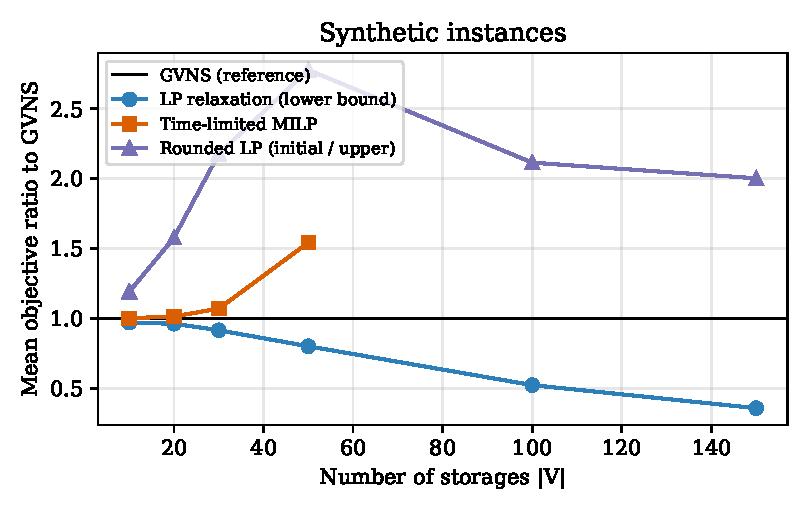
\includegraphics[width=\linewidth]{figs/synthetic_ratios.pdf}
  \caption{Synthetic instances (mean over instances of each size).}
  \label{fig:synth}
\end{subfigure}\hfill
\begin{subfigure}{0.49\textwidth}
  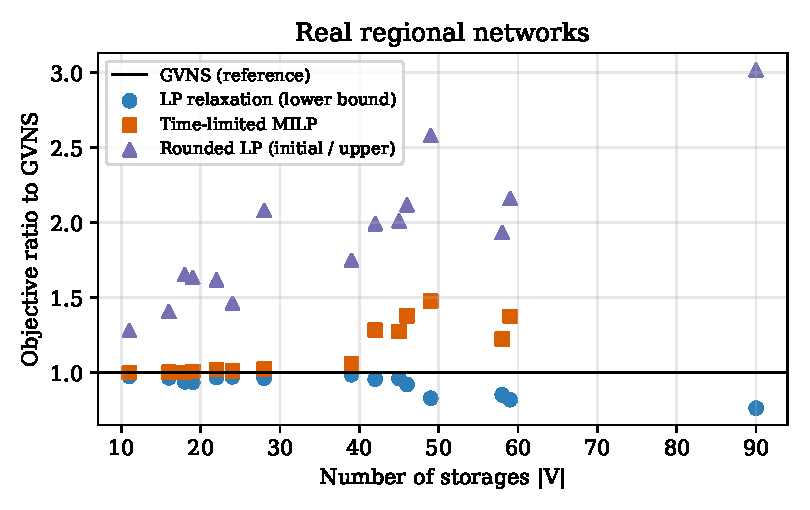
\includegraphics[width=\linewidth]{figs/real_ratios.pdf}
  \caption{Real-geometry regional networks.}
  \label{fig:real}
\end{subfigure}
\caption{Objective ratio of each reference method to GVNS as a function of
network size. Values below the GVNS reference line ($1.0$) are better than
GVNS; values above are worse.}
\label{fig:ratios}
\end{figure}

\begin{table}[t]
\centering
\caption{Synthetic results aggregated by network size (mean ratio to GVNS;
$n$ = number of instances). ``--'' indicates the time-limited MILP was not
obtainable.}
\label{tab:synth}
\small
\begin{tabular}{cccccc}
\toprule
$|V|$ & $n$ & Ratio LP-relax. & Ratio Rounded LP & Ratio MILP & mean time (s)\\
\midrule
10  & 10 & 0.970 & 1.191 & 1.001 & 424\\
20  & 7  & 0.962 & 1.577 & 1.014 & 1291\\
30  & 7  & 0.916 & 2.177 & 1.071 & 1705\\
50  & 5  & 0.802 & 2.776 & 1.543 & 4825\\
100 & 3  & 0.524 & 2.114 & --    & 11658\\
150 & 1  & 0.359 & 2.002 & --    & 18067\\
\bottomrule
\end{tabular}
\end{table}

\begin{table}[t]
\centering
\caption{Results on the real-geometry regional networks (ratios to GVNS).}
\label{tab:real}
\small
\begin{tabular}{lccccc}
\toprule
Network & $|V|$ & Ratio LP-relax. & Ratio Rounded LP & Ratio MILP & time (s)\\
\midrule
Belgium        & 11 & 0.977 & 1.282 & 1.000 & 609\\
Denmark        & 16 & 0.966 & 1.409 & 1.003 & 1041\\
Germany        & 18 & 0.939 & 1.655 & 1.003 & 1026\\
Hungary        & 19 & 0.937 & 1.636 & 1.009 & 488\\
Italy          & 22 & 0.968 & 1.618 & 1.022 & 2629\\
Netherlands    & 24 & 0.972 & 1.463 & 1.010 & 1792\\
Spain          & 28 & 0.964 & 2.081 & 1.026 & 3382\\
Sweden         & 39 & 0.987 & 1.749 & 1.062 & 4147\\
United Kingdom & 42 & 0.957 & 1.993 & 1.284 & 2671\\
California USA  & 45 & 0.962 & 2.011 & 1.274 & 4987\\
Georgia USA     & 46 & 0.922 & 2.119 & 1.380 & 2770\\
Illinois USA    & 49 & 0.830 & 2.582 & 1.478 & 3308\\
Ohio USA        & 58 & 0.853 & 1.934 & 1.226 & 3022\\
Texas USA       & 59 & 0.820 & 2.163 & 1.376 & 4087\\
Europe Russia  & 90 & 0.764 & 3.019 & --    & 11119\\
\bottomrule
\end{tabular}
\end{table}

\subsection{Solution analysis tool}
To inspect individual solutions in detail we developed an interactive web
application (Streamlit/Plotly) that loads any instance from the result corpus
and renders the network on its geographic layout: node sizes encode population
and capacity, edge widths encode vehicle counts and residual loads, and per-node
congestion ($overload_v$) is highlighted. The tool supports per-commodity path
inspection and aggregate statistics, which proved valuable both for debugging
the neighborhoods and for interpreting the structure of GVNS solutions.

\section{Conclusion}
We addressed the design of optimal logistic transport flows with nonlinear,
vehicle-induced edge costs and hard storage transshipment capacities. We gave
arc-based and path-based MILP models and their linear relaxation, and proposed a
GVNS that operates in the path space through three problem-specific
neighborhoods: reload-aware shortest paths, partially loaded edges, and detours
around congested storages. To enable evaluation in the absence of public
benchmarks, we built a generator of realistic logistic networks calibrated on
real road graphs and reproducing their near-planar topology, Zipf city sizes
and gravity-model demand.

On $34$ synthetic and $15$ real-geometry instances of up to $150$ storages,
GVNS consistently produced solutions close to the LP lower bound and clearly
better than both the rounded-relaxation upper bound and a time-limited exact
solver run for a comparable budget; the relative gap to the lower bound grows
with size, as expected from the exploding path space. Future work includes
refining and extending the neighborhoods, integrating column-generation pricing
to feed the path pool, and validating the approach on operational data from
real logistic systems.

\begin{thebibliography}{99}
\small
\bibitem{barnhart1998} C.~Barnhart, E.~L.~Johnson, G.~L.~Nemhauser,
M.~W.~P.~Savelsbergh, P.~H.~Vance. Branch-and-Price: Column Generation for
Solving Huge Integer Programs. \textit{Operations Research}, 46(3):316--329,
1998.
\bibitem{crainic2015} T.~G.~Crainic, M.~Gendreau, J.~M.~Farvolden.
Metaheuristics for Multi-Commodity Flow Problems. \textit{Parallel Computing},
41:1--15, 2015.
\bibitem{masri2015} H.~Masri, S.~Krichen, A.~Guitouni. A multi-start variable
neighborhood search for solving the single path multicommodity flow problem.
\textit{Applied Mathematics and Computation}, 251:132--142, 2015.
\bibitem{amous2017} M.~Amous, S.~Toumi, B.~Jarboui, M.~Eddaly. A variable
neighborhood search algorithm for the capacitated vehicle routing problem.
\textit{Computers \& Operations Research}, 88:234--248, 2017.
\bibitem{hansen2019} P.~Hansen, N.~Mladenovi\'c. Variable Neighborhood Search.
In \textit{Handbook of Metaheuristics}, 3rd ed., Springer, 57--97, 2019.
\bibitem{hansen2017} P.~Hansen, N.~Mladenovi\'c, R.~Todosijevi\'c, S.~Hanafi.
Variable neighborhood search: Basics and variants. \textit{EURO Journal on
Computational Optimization}, 5(3):423--454, 2017.
\bibitem{karakostas2019} P.~Karakostas, A.~Sifaleras, M.~C.~Georgiadis. A
general variable neighborhood search-based solution approach for the
location-inventory routing problem with distribution outsourcing.
\textit{Computers \& Chemical Engineering}, 126:263--279, 2019.
\bibitem{mjirda2014} A.~Mjirda, B.~Jarboui, N.~Mladenovi\'c, C.~Wilbaut,
S.~Hanafi. A general variable neighbourhood search for the multi-product
inventory routing problem. \textit{Int.\ J.\ of Production Research}, 2014.
\bibitem{osm} OpenStreetMap. \url{https://www.openstreetmap.org} (accessed
2026-04-11).
\bibitem{gabaix1999} X.~Gabaix. Zipf's Law for Cities: An Explanation.
\textit{Quarterly Journal of Economics}, 114(3):739--767, 1999.
\bibitem{gastner2006} M.~T.~Gastner, M.~E.~J.~Newman. The spatial structure of
networks. \textit{The European Physical Journal B}, 49(2):247--252, 2006.
\bibitem{barthelemy2011} M.~Barth\'elemy. Spatial networks. \textit{Physics
Reports}, 499(1--3):1--101, 2011.
\bibitem{kirkley2018} A.~Kirkley, H.~Barbosa, M.~Barthelemy, G.~Ghoshal. From
networks to optimal higher-order models of complex systems. \textit{Nature
Physics}, 14:250--258, 2018.
\bibitem{wilson1967} A.~G.~Wilson. A statistical theory of spatial distribution
models. \textit{Transportation Research}, 1(3):253--269, 1967.
\end{thebibliography}

\end{document}
